% ---------------------------------------------------------------------------- %
\chapter{Fundamentos}
\label{cap:fundamentos}
% ---------------------------------------------------------------------------- %

Para se criar e treinar uma inteligência artificial, diversos arcabouçous são necessários. Por um lado, existe a parte teórica e matemática na qual a inteligência se baseia para aprender. Por outro, do lado computacional, existem as bibliotecas que auxiliam no desenvolvimento, efetuando as contas necessárias e, neste trabalho em particular, emulando o jogo que serve de ambiente para o aprendizado.
Este capítulo tem o intuito de familiarizar o leitor com a teoria e as ferramentas utilizadas no treinamento da inteligência artificial deste trabalho.

% ---------------------------------------------------------------------------- %
% https://en.wikipedia.org/wiki/Asteroids_(video_game)
% https://en.wikipedia.org/wiki/Golden_age_of_arcade_video_games
% https://www.arcade-museum.com/game_detail.php?game_id=6939
% https://www.ranker.com/list/the-most-popular-golden-age-arcade-games/video-games-lists
\section{Asteroids}
\label{sec:asteroids}

Asteroids é um jogo de fliperama do gênero shooter (jogo eletrônico de tiro) lançado em novembro de 1979 pela então desenvolvedora de jogos eletrônicos Atari Inc, atualmente conhecida apenas como Atari. O jogo foi inspirado por Spacewar!, Computer Space, Space Invaders, e Cosmos, sendo este último um jogo não finalizado.

O jogador controla uma nave espacial que se encontra em um campo de asteróides e precisa atirar para destruir todos enquanto evita colisões com os mesmos. A dificuldade aumenta conforme o número de asteróides na tela aumenta.
Diversas versões deste jogo foram criadas ao longo dos anos. Além das diferenças gráficas, as mudanças incluem naves espaciais inimigas que atiram contra o jogador, e tamanhos e formatos diferentes que os asteróides podem ter.
Asteroids é considerado um dos primeiros grandes sucessos da era de ouro dos jogos de fliperama, época em que os jogos eletrônicos se estabeleceram como uma força dominante na cultura popular. 

Para este trabalho, Asteroids foi emulado utilizando a plataforma Gym-Retro da companhia de pesquisas de inteligência artificial OpenAI. Todas as informações sobre o jogo apresentadas a seguir referem-se a tal versão.
Para o aprendizado da inteligência artificial, não há naves inimigas e os asteróides podem assumir três tamanhos e três formatos distintos. Os tamanhos são grande (inicial), médio e pequeno, enquanto os formatos são consideravelmente parecidos.
Há cinco comandos disponíveis: mover-se para frente, girar a nave no sentido horário, girar a nave no sentido anti-horário, atirar para frente, e entrar no hiper espaço. Mover-se para frente e girar no sentido horário ou anti-horário são as principais formas de movimento disponíveis ao jogador, e atirar serve para destruir os asteróides. Mover-se no hiper espaço consiste em fazer a nave desaparecer e, depois de alguns instantes, reaparecer em um local aleatório da tela. Há o risco de reaparecer em cima de um asteróide e, com isso, ter a nave destruída e perder uma vida.
A nave possui aceleração e desaceleração - ou seja, inércia. Em outras palavras, mesmo que o jogador deixe de pressionar o botão de mover-se para frente, ele continuará em movimento por um curto período de tempo antes de parar por completo. Isso gera um grau a mais de complexidade, pois faz com que manobras de esquiva e curvas sejam mais difíceis de serem devidamente executadas.

% ---------------------------------------------------------------------------- %
% https://github.com/openai/retro
% https://blog.openai.com/gym-retro/
% https://openai.com/
% https://gym.openai.com/
\section{Gym-Retro}
\label{sec:gymretro}

Gym-Retro é uma plataforma para pesquisa de aprendizado por reforços e generalização em jogos desenvolvida e mantida pela empresa de pesquisas em inteligência artificial OpenAI. O lançamento mais recente inclui, como ambientes para o desenvolvimento de IA, jogos do Sega Genesis, Sega Master System, Nintendo Entertainment System (NES), Super Nintendo Entertainment System (SNES) e Nintendo Game Boy, além de suporte preliminar para Sega Game Gear, Nintendo Game Boy Color, Nintendo Game Boy Advance e NEC TurboGrafx. Em qualquer um desses consoles, a ROM (Read Only Memory) do jogo é necessária.
Apesar de não ter sido utilizada neste trabalho, a plataforma disponibiliza uma ferramente que permite criar save states (salvar um estado a partir do qual é possível continuar o jogo), encontrar locais da memória, criar cenarios para o agente resolver, gravar e passar arquivos de vídeo, dentre outras funcionalidades.

Gym-Retro baseia-se na ferramenta Gym, desenvolvida e mantida pela OpenAI, que também tem como objetivo pesquisas em aprendizado por reforço, mas não apenas para jogos.
Esta ferramenta foi utilizada por ter suporte para desenvolvimento de aprendizado para o jogo Asteroids e ser de fácil uso. A plataforma permite a entrada de oito ações diferentes: UP, DOWN, LEFT, RIGHT, BUTTON, SELECT, RESET, null, sendo que a ação realiada por cada botão varia de acordo com o jogo. Como descrito anteriormente, Asteroids utiliza apenas cinco deles: UP (mover-se para frente), DOWN (mover-se no hiper espaço), RIGHT (girar no sentido horário), LEFT (mover-se no sentido anti-horário), e BUTTON (atirar). Os demais botões (SELECT e RESET) possuem funções relacioandas ao sistema e não ao jogo, e null é não realizar nenhuma ação.

% ---------------------------------------------------------------------------- %
% https://en.wikipedia.org/wiki/TensorFlow
% https://github.com/tensorflow/tensorflow
% https://www.tensorflow.org/
\section{TensorFlow}
\label{sec:tensorflow}

TensorFlow é um arcabouço de código aberto para computações numéricas de alta performance, desenvolvido e mantido pela Google. Seu núcleo de computação numérica flexível permite o uso da biblioteca em diversos campos da ciência. Oferece, em particular, grande suporte a aprendizado de máquina e deep learning.
Esta ferramenta foi utilizada por oferecer uma API em Python estável, ter grande suporte, comunidade ativa, e ser de código aberto.
Apesar de não ter sido utilizado, esta biblioteca também possui uma ferramenta de visualização de dados chamada TensorBoard.

% ---------------------------------------------------------------------------- %
% RUSSEL, Stuart Jonathan and NORVIG, Peter - Artificial Intelligence: a mordern approach
% 
\section{Inteligência artificial (IA)}
\label{sec:ia}

Inteligência artificial (IA) é um dos campos mais recentes de ciência e engenharia, tendo trabalhos no assunto sendo iniciados pouco depois da Segunda Guerra Mundial. Atualmente, ela é composta por diversos campos menores de estudo, podendo ser mais genérico, como aprendizado e percepção, até mais específico, como a capacidade de jogar um jogo, provar teoremas matemáticas, ou dirigir um carro em uma via movimentada.
No livro Artificial Intelligence: A Morden Approach, de Stuart Jonathan Russel e Peter Norvig, oito definições são apresentadas em uma tabela de duas linhas por duas colunas. A linha de cima define processo de pensamento (\textit{thought process}) e raciocínio (\textit{reasoning}), enquanto a linha de baixo define comportamento (\textit{behaviour}). Além disso, a coluna da esquerda mede o grau de fidelidade da inteligência quando comparado com performance humana, enquanto a da direita mede a racionalidade da performance - ou seja, se toma a ação "correta" dado o que o sistema sabe.

\begin{tabular}{| p{7cm} | p{7cm} |}
  \hline
  \textbf{Pensando como um humano} & \textbf{Pensando racionalmente} \\ \hline
  \textit{O empolgante novo esforço de fazer computadores pensarem, serem máquinas com mentes, no sentido completo e literal da expressão} \newline (Haugeland, 1986) & \textit{O estudo das faculdades mentais através de modelos computacionais} \newline (Charniak \& McDermott, 1985) \\ & \\ \textit{[A automação de] atividades que são associadas ao pensamento humano, como resolução de problemas, tomada de decisão, aprendizado, ...} \newline (Hellman, 1978) & \textit{O estudo das computações que tornam possível a percepção, razão, e ação} \newline (Winston, 1992) \\ \hline
  \textbf{Agindo como um humano} & \textbf{Agindo racionalmente} \\ \hline
  \textit{A arte de criar máquinas capazes de realizar funções que requerem inteligência quando feitas por pessoas} \newline (Kurzweil, 1990) & \textit{Inteligência computacional é o estudo do design de agentes inteligentes} \newline (Poole \textit{et at}, 1998) \\ & \\ \textit{O estudo de como fazer os computadores fazerem coisas que, no momento, pessoas fazem melhor} \newline (Rich and Knight, 1991) & \textit{IA... está relacionada a comportamento inteligente em objetos} \newline (Nilsson, 1998) \\ \hline
\end{tabular}

Em linhas gerais, as definições da coluna da esquerda dizem respeito a uma inteligência artificial que se pareça com um humano, enquanto as da direita sobre uma inteligência artificial que toma ações visando estar correta e a atingir o melhor resultado possível. Pela natureza de \textit{Deep Q Learning}, tipo de aprendizado utilizado neste trabalho, o foco será em agir racionalmente, ou seja, tomar ações que são mais prováveis de retornar a melhor recompensa.

%Agindo como um humano: Teste de Turing. Envolve processamento de linguagem natural, representação de conhecimento, raciocínio automatizado, aprendizado de máquina e, no caso do teste de Turing total, visão computacional e robótica. Contudo, cientistas dedicaram pouco tempo em passar nesse teste, pois acreditam ser mais importante estudar os princípios da inteligência do que duplicar uma.

%Pensando como um humano: unindo computação com psicologia, a modelagem cognitiva busca expressar a teoria de como a mente funciona em um programa de computador. Duas vertentes surgiram a partir dessa abordagem: um programa tem bons resultados em uma tarefa e, portanto, é um bom modelo da performance humana, e vice-versa. Com essa separação, foi possível as duas linhas progredirem mais rapidamente, uma contribuindo com a outra.

%Pensando racionalmente: Lógica, leis do pensamento. Esta abordagem busca criar uma inteligência artificial que consiga sempre resolver um problema contanto que as premissas corretas sejam dadas. Seguindo passos lógicas, a inteligência chega a conclusões apenas se forem consequências lógicas do que já se sabe e/ou foi concluído até o momento.

%Agindo racionalmente: Um agente racional é esperado que aja de forma que atinja o melhor resultado possível ou, se houver incerteza, o melhor resultado esperado. Esta abordagem pode ser considerada um passo além das leis do pensamento, pois consegue tomar decisões quando necessário mesmo que não haja uma escolha provadamente correta.

\subsection{Aprendizagem por reforço}
\label{sec:rl}

Aprendizagem por reforço (\textit{reinforcement learning}) é uma das técnicas de aprendizado de inteligência artificial e a utilizada neste trabalho.



\begin{displayquote}
  \textit{Game Design é o ato de decidir como um jogo deve ser.}\footnote{Tradução livre feita pelo autor}
\end{displayquote}

\begin{lstlisting}
  while (true)
  {
    processInput();
    update();
    render();
  }
\end{lstlisting}

% ---------------------------------------------------------------------------- %
\section{Técnicas}
\label{sec:tecnicas}

Apesar de grande parte do desenvolvimento de \textit{PsyChO: The Ball} ter sido feita apenas por uma pessoa, foi muito benéfica a utilização de sistemas de versionamento que ajudam tanto na centralização de todo o código do jogo, facilitando na transição entre ambientes de trabalho, quanto na possibilidade de guardar versões antigas e resgatar códigos passados quando necessário. Durante todo o desenvolvimento de \textit{PsyChO: The Ball} foi utilizado um sistema de controle de versão para código e nele se encontram todas as versões de lançamento do jogo.

Uma boa prática na produção de um jogo, seja esse comercial ou um projeto pessoal, é a de lançamentos, ou \textit{releases}, constantes. O propósito disto é ter, periodicamente, \textit{releases} de versões estáveis e jogáveis do jogo, de forma que outras pessoas possam jogar e dar \textit{feedback} frequente, assim ajudando no encaminhamento do projeto. Essa técnica é muito comum em metodologias ágeis de desenvolvimento de software e essa linha de pensamento foi o que guiou todo o desenvolvimento de \textit{PsyChO: The Ball}.

Inicialmente foi utilizado o sistema \textit{Kanban}, uma abordagem moderna de conceitos ágeis muito comum em empresas ou grupos de desenvolvimento de software. Kleber Bernardo, especialista em métodos ágeis, descreve bem a metodologia em um artigo no site Cultura Ágil \cite{kleberkanban}:

\begin{displayquote}
  \textit{O Kanban lhe ajuda a assimilar e controlar o progresso de suas tarefas de forma visual. É, normalmente, utilizado um quadro branco com alguns pequenos papéis (Post-it) colados, esses papéis representam as suas tarefas, ao termino de cada tarefa o papel é puxado para a etapa seguinte até que a mesma seja finalizada. Ao olhar para um quadro Kanban é fácil enxergar como o trabalho seu e de sua equipe fluem, permitindo não só comunicar o status, mas também dar e receber feedbacks.}
\end{displayquote}

\begin{figure}[h!]
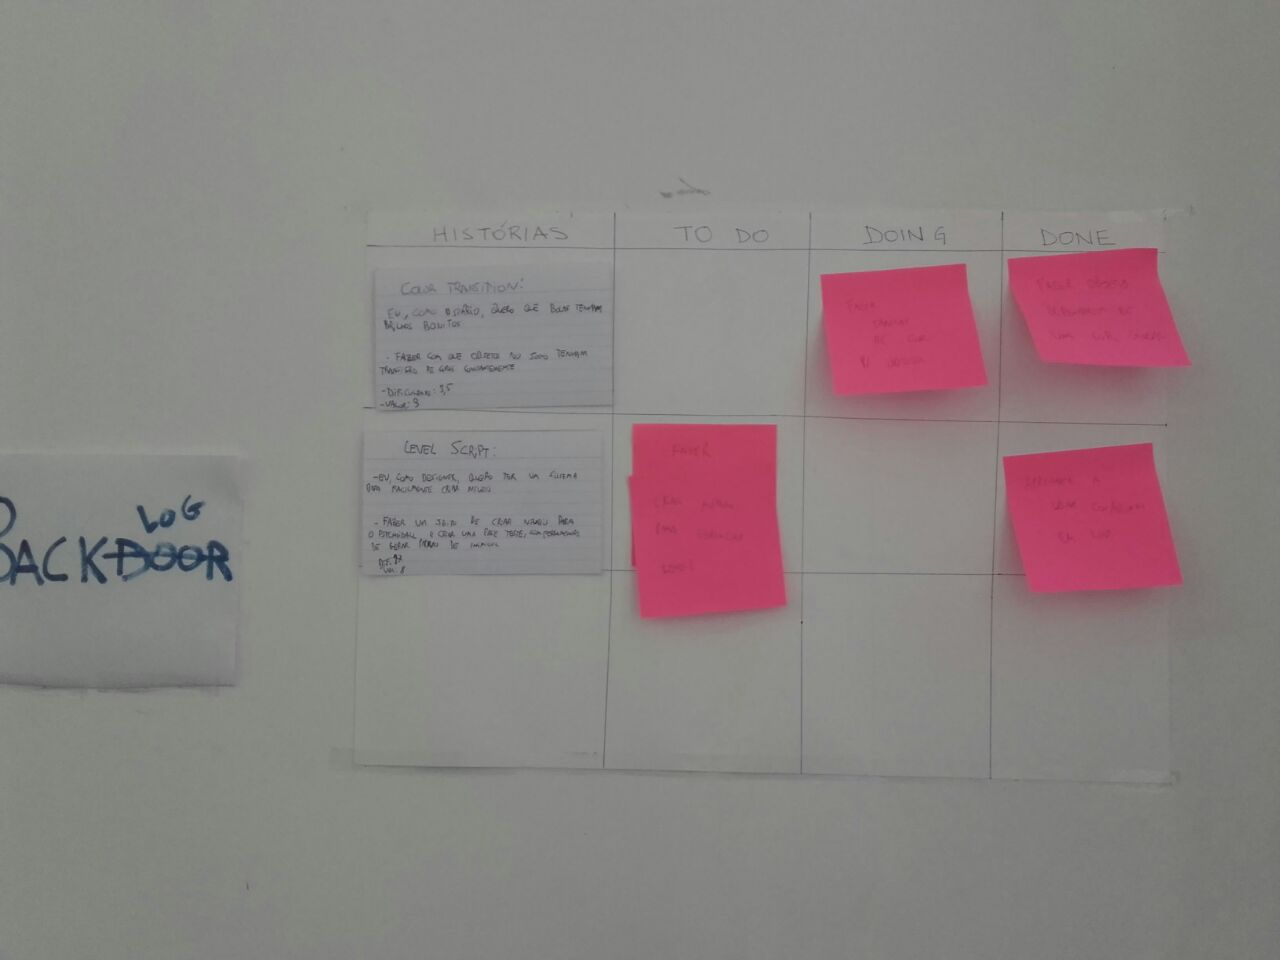
\includegraphics[scale=.3]{kanban}
\centering
\caption{Kanban utilizado durante o desenvolvimento de \textit{PsyChO: The Ball}}
\end{figure}

Entretanto, após alguns meses utilizando essa técnica, o tempo gasto em sua manutenção acabou se tornando mais trabalhoso do que produtivo para o projeto e seu uso foi decaindo. Desta forma o \textit{Kanban} foi substituido por várias pequenas técnicas ágeis, como lançamentos frequentes do jogo, \textit{sprints} (onde era determinado um prazo de uma ou duas semanas para terminar funcionalidades no jogo) e constantes re-avaliações com consulta de \textit{feedback}.

Por último, uma técnica muito presente no desenvolvimento do jogo foi a utilização de documentação para marcar mudanças e melhorias no projeto. Os dois documento mais importantes são o \textit{DEVLOG}\footnote{https://github.com/uspgamedev/Project-Telos/blob/dev/docs/DEVLOG.md} e \textit{CHANGELOG}\footnote{https://github.com/uspgamedev/Project-Telos/blob/dev/docs/CHANGELOG.md}. O \textit{DEVLOG} foi um necessário para mostrar o progresso e tempo gasto no projeto, enquanto este fazia parte da disciplina \textit{MAC0214 Atividade Curricular em Cultura e Extensão}. Nele existem várias entradas detalhando atividades feitas no jogo durante o desenvolvimento. O \textit{CHANGELOG} por outro lado serve para marcar lançamentos do jogo, descrevendo \textit{features} novos adicionados em cada \textit{sprint} feito. Ambos documentos foram de grande utilidade no início do desenvolvimento de \textit{PsyChO: The Ball}, pois exibem concretamente o fluxo de progresso na criação do jogo.

% ---------------------------------------------------------------------------- %
\section{Ferramentas}
\label{sec:ferramentas}

Uma das escolhas feitas para o desenvolvimento de \textit{PsyChO: The Ball} foi a utilização exclusiva de \textit{Software Livre}. Essa decisão se deu tanto pela liberdade que essas ferramentas permitem em sua utilização, quanto pelo objetivo de incentivar mais o uso desse tipo de software, mostrando que é tão eficiente quanto o uso de software proprietário. Assim, como critério de escolha para cada área de desenvolvimento do jogo, foi determinado algum software livre que tenha uma comunidade ativa (para a solução de problemas e disponibilidade de bibliotecas), constante atualização de suas funcionalidades, versões estáveis e uma recomendação de seu uso no desenvolvimento de jogos.

O arcabouço utilizado no desenvolvimento de \textit{PsyChO: The Ball} foi a \textit{Love2d} ou \textit{LÖVE}\footnote{https://love2d.org/}, uma \textit{framework} gratuita que utiliza a linguagem \textit{Lua}\footnote{https://www.lua.org/portugues.html}.

Como sistema de controle de versão foi utilizado \textit{Git}\footnote{https://git-scm.com/} através da plataforma de uso grátis \textit{Github}\footnote{https://github.com/}.

Para a produção de música foi utilizado \textit{LMMS}\footnote{https://lmms.io/}, um software livre gratuito para manipulação e criação de sons.

Por último, para manipulação de imagens, foi utilizada a ferramenta \textit{Gimp}\footnote{https://www.gimp.org/}.

\begin{figure}[h!]

\includegraphics[scale=.5]{icons}
\centering
\caption{Da esquerda pra direita, ícones de \textit{LÖVE}, \textit{Lua}, \textit{Git}, \textit{Github}, \textit{LMMS} e \textit{Gimp}}
\end{figure}

Dentre essas ferramentas, vale ressaltar um ponto muito interessante do arcabouço \textit{LÖVE}: seu \textit{gameloop} tem o diferencial de deslocar todas as verificações de \textit{input} do usuário como \textit{callbacks assíncronos}. Estes são funções que a própria \textit{framework} vai chamar quando ocorrer algum \textit{input} do usuário, como quando ele pressionar um botão do teclado ou mover o mouse. Através de subrotinas, o arcabouço está constantemente aguardando sinais que ativem essas funções e assim o desenvolvedor não precisa se preocupar em lidar com otimização ou código confuso na hora de esperar e tratar comandos dados pelo usuário. Isso foi uma grande vantagem que determinou a escolha dessa ferramenta na produção de \textit{PsyChO: The Ball}.

% ---------------------------------------------------------------------------- %
